\documentclass[Afour,sagev,times]{sagej}
\usepackage{moreverb,url}
\usepackage{epstopdf}
\usepackage[colorlinks,bookmarksopen,bookmarksnumbered,citecolor=red,urlcolor=red]{hyperref}
\usepackage{graphicx}
\usepackage{subcaption}
\newcommand\BibTeX{{\rmfamily B\kern-.05em \textsc{i\kern-.025em b}\kern-.08em
T\kern-.1667em\lower.7ex\hbox{E}\kern-.125emX}}
\def\volumeyear{2016}
\usepackage[utf8]{inputenc}
\usepackage[T1]{fontenc}
\usepackage{amsmath, xparse}
\usepackage{algorithm}
\usepackage{algorithmic}
\usepackage{graphicx}
\graphicspath{ {pics/} }
\DeclareMathOperator{\sech}{sech}
\newcommand{\squeezeup}{\vspace{-4mm}}
\usepackage{amsmath}
\usepackage{balance}
\usepackage{lastpage}
\usepackage{array}
\usepackage{tabularx}
\usepackage{longtable}
\makeatletter
    \def\balanceissued{unbalanced}%flag to indicate if \balance has been used
    \let\oldbibitem\bibitem
    \def\bibitem{%
        \ifnum\thepage=\lastpage@lastpage%
            \expandafter\ifx\expandafter\relax\balanceissued\relax\else%
                \balance%
                \gdef\balanceissued{\relax}\fi%
            \else\fi%
        \oldbibitem}
\makeatother
\usepackage{natbib}
\setcitestyle{square, comma, numbers,sort&compress, super}
\setcitestyle{super}
\newcommand*{\citen}[1]{%
  \begingroup
    \romannumeral-`\x % remove space at the beginning of \setcitestyle
    \setcitestyle{numbers}%
    \cite{#1}%
  \endgroup   
}
\begin{document}

\runninghead{Ch.Narendra Kumar ~and
        ~K P Sinhamahapatra}

\title{The Effects of Spacing to Diameter Ratio on Mixing Characteristics of Twin Jets}

\author{Ch.Narendra Kumar and K P Sinhamahapatra }

\affiliation{Department of Aerospace Engineering, Indian Institute of Technology
Kharagpur, Kharagpur, India}

\corrauth{Ch.Narendra Kumar, Department of Aerospace Engineering, Indian
Institute of Technology Kharagpur, Kharagpur, India.}

\email{chnarendrakumar06@gmail.com}

\begin{abstract}
In this paper, the effects of spacing to diameter (\textit{S/D}) ratio and orientation on mixing properties of circular and elliptical twin jets are investigated numerically at four different~\textit{S/D}~ratios of 0.25, 0.50, 0.75, and 1.0, respectively. The numerical simulations of twin jets are carried out with jet Mach number of 0.8 using the Shear Stress Transport (\textit{SST})~\textit{K-$\omega$}~turbulence model. The results show that near the orifice exit, the twin jets are issuing into ambient conditions separately and resemble a free jet, leading to a potential core length independent of~\textit{S/D}. The merging and combined point locations change linearly from the exit with an increasing~\textit{S/D}~ratio. The decay rate is higher for Twin Ellipse Minor than those in Twin Circle and Twin Ellipse Major, verified by a shorter converging region. The jet mixing is superior for twin minor elliptical configuration compared to twin circle and twin major jets.
\end{abstract}
\keywords{Twin jets, Mixing, ANSYS-Fluent, Potential core, Combined Point}

\maketitle

\section{Introduction}
Since several years, twin jets mixing behaviour has been investigated experimentally and numerically. The closely spaced twin jets are practically used in military and fighter aircraft for stealth applications. A better idea and understanding of the flow field of a twin jet can consequently help in controlling the impact of exhaust pollutants. The past research identified that the properties of mixing and turbulent intensities of the circular and non-circular cross sections are dependent on exit Reynolds number (Re), nozzle topology, and \textit{S/D} between the nozzles \cite{deo2008influence,harima2005turbulent}. Previous studies on elliptic, triangular, rectangular, and star-shaped nozzles help identify the underlying mechanism involved with the axis-switching phenomena \cite{mi2010statistical,quinn2007experimental,quinn2005measurements,xu2014effect,aleyasin2015low}. It is a streamwise location where the major and minor axis half velocity widths coincide and is the leading cause of higher mixing in non-circular jets \cite{aleyasin2015low}.  

Understanding the flow properties of twin jets is more complicated than the single jet due to its communal interaction between the two individual jets. The schematic diagram of the twin jet flow field is shown in Fig. \ref{fig:twinjet flow}. A twin jet system consists of three regions: a converging region, a merging region, and a combined region. As Miller and Comings [8] discussed in their investigation on plane twin jets, negative gauge static pressures are observed in the near field of a twin jet, making the two jets connect in the downstream. Two individual jets experience a recirculation zone near the nozzle exit that causes negative jet velocity in the symmetry plane \cite{miller1960force,lin1990investigation}. Thus, in some twin jets investigations, the merging point is defined as the point where the streamwise velocity changes its sign from negative to positive \cite{lin1990investigation}. However, the definition is not valid for small spacing distances between the nozzles as they are ineffective in developing the recirculation region at the nozzle exit. Thus a different understanding of defining the merging point (\textit{X${}_{mp}$}) has been adopted by different authors. In this paper, following Refs. \citen{laban2019experimental} and \citen{aleyasin2019statistical}, the merging point is defined as the location at which the streamwise velocity increases rapidly towards an asymptote. The converging region is defined as the region between the nozzle exits to the merging point location. The region between the merging point and the combined point is termed as the merging region. After the merging region, the two jets behave like a single jet, and velocity profiles look similar. The location at which twin jets fully merge as a single jet is called a combined point (\textit{X${}_{cp}$}), and the region after this point is called a combined region. 
%%%%%%%%%%%%%%%%%%%%%%%%%%%%%%%%%%%%%%%%%%%%%%%%%%%%%%%%%%%%%%%%%%%%%%%%%%%%%%%%%%%%%%%%%%%%%%%%
\begin{figure}[h]
\centering
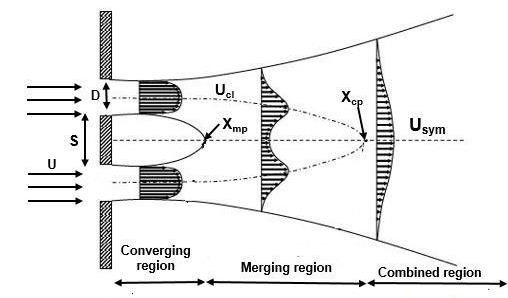
\includegraphics[width=3.4in]{twin jet flow field.png}
\caption{Schematic flow structure of a twin jet }
\label{fig:twinjet flow}
\end{figure}
%%%%%%%%%%%%%%%%%%%%%%%%%%%%%%%%%%%%%%%%%%%%%%%%%%%%%%%%%%%%%%%%%%%%%%%%%%%%%%%%%%%%%%%%%%%%%%%%

For several years now, both experimental and numerical researches are ongoing on twin jets to identify the optimal nozzle configurations and improving mixing efficiency. Lin and Sheu \cite{lin1990investigation} examined the impact of spacing on the merging point of twin jets in the range of \textit{S/D} $\mathrm{<}$ 30 and measured the centerline velocity variation in the mixing and combined regions. Lin and Sheu \cite{lin1990investigation} formulated a relationship to find the X${}_{mp}$ location in terms of \textit{S/D}, the relation predicts the \textit{X${}_{mp}$} location with an accuracy of $\mathrm{\pm}$ 12\%. The relationship does not apply for \textit{S/D}$\mathrm{<}$30. This is mainly due to the fact that for \textit{S/D}$\mathrm{>}$30 the merging point occurs far enough so that the jet exit conditions, such as the turbulent intensity, do not affect \textit{X${}_{mp}$/D}.
%%%%%%%%%%%%%%%%%%%%%%%%%%%%%%%%%%%%%%%%%%%%%%%%%%%%%%%%%%%%%%%%%%%%%%%%%%%%%%%%%%%%%%%%%%%%%%%%
\begin{equation}\label{eq1}
%\begin{split}
\textit{S/D = -18.73+2.085(X${}_{mp}$/D)}
%\end{split}
\end{equation} 
Where \textit{X${}_{mp}$}${}_{\ }$is the axial location of the merging point.
%%%%%%%%%%%%%%%%%%%%%%%%%%%%%%%%%%%%%%%%%%%%%%%%%%%%%%%%%%%%%%%%%%%%%%%%%%%%%%%%%%%%%%%%%%%%%%%%
Anderson and Spall \cite{anderson2001experimental} studied the influences of spacing variation on combined and merging points of twin jets. It was observed that the turbulent intensities of the combined jet increase progressively by increasing the \textit{S/D} ratio. M. Mosavati et al. \cite{mosavati2021characteristics} investigated the round and square twin jets issuing into a narrow cavity using the Reynolds stress turbulence model at four different \textit{S/D} ratios and reported that the nozzle shape of the square and round twin jets does not significantly affect the jet decay. The effects of nozzle orientation on mixing and turbulent properties of elliptical twin jets were studied experimentally by E.M. Morris et al. \cite{morris2021particle}. It was found that the velocity does not vary significantly with orientation. Still the spread rate was higher for the twin minor nozzle in the jet exit. Laban et al. \cite{laban2019experimental} investigated the spacing distance effects on circular twin jets at a fixed Re. It was noted that an increment in spacing reduced the jet spread rate and a decrease in turbulent properties.  

It appears that in the past, the extent of literature on the detailed numerical simulations of three- dimensional jet flows was minimal.\textbf{ }This is understandable in view of the severe computational resources required for such simulations. However, the present-day development of supercomputers and high-performance computing techniques enabled numerical studies on turbulent jets significantly. Anderson and Spall \cite{anderson2001experimental} evaluated the turbulence models \textit{K-$\varepsilon$}, \textit{SST K-$\omega$}, and \textit{RSM} in predicting the mixing properties of twin jets. They suggested that \textit{K-$\omega$} and \textit{RSM} models are suitable enough for the simulation of twin jets. A Valencia and Maximo Leon \cite{valencia2021analysis} studied the single and twin jets under expanded conditions using \textit{URANS }simulations at different spacing distances. They found that injecting the same mass flow rate in single and twin jets increases the potential core of the individual jet and combined core. Shorter potential core length and increase in mixing levels are observed for larger spacing conditions. Nasr and Lai \cite{nasr1997comparison} also correlated the ability of standard \textit{K-$\varepsilon$}, \textit{RNG}, and \textit{RSM} turbulence models for 2d parallel-twin jets. It was observed that the RSM model has the closest results to the experimental than the other two models, and slightly over prediction is found for the \textit{K-$\varepsilon$} method over experimental results. To investigate the flow properties of a cross-shaped orifice, Amina Meslem et al. \cite{meslem2014comparison} simulated seven turbulence models, i.e., linear (Low Reynolds and Renormalization Group), nonlinear (quadratic and cubic) \textit{K-$\varepsilon$} turbulence models, \textit{K-$\omega$, SST K-$\omega$} turbulence models, and \textit{RSM}.  The authors reported that \textit{SST K-$\omega$} is accurate in predicting the mean flow characteristics in the near field, axis switching phenomenon, streamwise velocity, and vorticity field. In contrast, the other turbulence models are not able to predict jet characteristics accurately. In recent years, several researchers suggested that \textit{RANS} modelling is accurate enough to understand the mixing properties of jets \cite{lin1990investigation,anderson2001experimental}. Therefore the present study is an attempt to evaluate the \textit{RANS-}based \textit{SST K-$\omega$} turbulence model to predict the effects of \textit{S/D} ratio, nozzle orientation, and geometry on the mixing properties of turbulent free, plane, parallel twin jets. The numerical simulations are performed in finite volume-based computational fluid dynamic (\textit{CFD}) solver ANSYS Fluent v19.2. Furthermore, few experimental and numerical results are compared with the present numerical findings. 

\section{Problem Description}

Numerical simulations that are performed in the present investigation for circular orifice is the one Anderson and Spall \cite{anderson2001experimental} studied experimentally. For the present \textit{RANS}-based numerical study, three jet geometries have been chosen with exit cross sections of circular and elliptical shapes. The elliptical orifice is oriented either along the major axis plane (Twin Ellipse Major) or the minor axis plane (Twin Ellipse Minor) to determine the orientation effects on mixing. The exit diameter (\textit{D}) of the circular orifice is 15 mm, and the elliptical orifice major (2ae) and minor (2be) axes lengths are 20 mm and 11.25 mm, respectively. Fig. \ref{fig:models} shows the geometrical shapes with relevant notations. All the chosen jet models have an exit area of 176.625 mm${}^{2}$ and a 0.06 kg/sec mass flow rate at nozzle exit. The chosen models are simulated numerically for both single and twin jets at four different \textit{S/D} ratios of 0.25, 0.50, 0.75 and 1.0 with jet operating Mach number (\textit{M}) of 0.8. 
%%%%%%%%%%%%%%%%%%%%%%%%%%%%%%%%%%%%%%%%%%%%%%%%%%%%%%%%%%%%%%%%%%%%%%%%%%%%%%%%%%%%%%%%%%%%%
\begin{figure}[h]
\centering
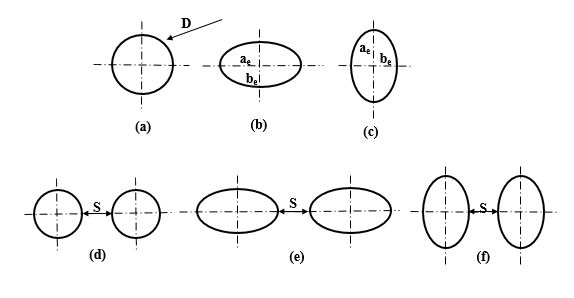
\includegraphics[width=3.4in]{geometrical models.png}
\caption{(a) Single Circle, (b) Single Ellipse Major, (c) Single Ellipse Minor, (d) Twin Circle, (e) Twin Ellipse Major, (f) Twin Ellipse Minor orifice configurations}
\label{fig:models}
\end{figure}
%%%%%%%%%%%%%%%%%%%%%%%%%%%%%%%%%%%%%%%%%%%%%%%%%%%%%%%%%%%%%%%%%%%%%%%%%%%%%%%%%%%%%%%%%
\section{Numerical Methodology}

\subsection{Computational Solver}
In the present investigation, a finite volume method \cite{anderson1995computational} based commercial software package, ANSYS Fluent with \textit{SST K-$\omega$} turbulence model was utilised to simulate the steady state compressible flow issuing from single and twin jet orifice plates. The pressure-based coupled solver is used for steady-state \textit{RANS} simulations. Air, as an ideal gas is taken as the jet fluid and viscosity is calculated using Sutherland three coefficient method. The under-relaxation factors for the momentum and pressure were defined as 1 and 1, respectively. To discretize the convection terms bounded QUICK scheme \cite{leonard1979stable} is used. Viscous terms are solved by second order central differencing scheme, and SIMPLEC procedure is followed for the pressure--velocity coupling with skewness correction of 1 \cite{patankar2018numerical}. A double-precision solver setting was followed to approximate the computer-generated round-off errors. Simulations were iterated till the convergence of results is achieved.  The residuals are considered to be converged when absolute values of the pressure, temperature and different components of velocity are below 10${}^{-6\ }$in the iterative solution procedure. The turbulence model employed in the present numerical study is the \textit{SST K-$\omega$} model, where turbulent kinetic energy is denoted by \textit{K} and specific rate of dissipation is denoted by \textit{$\omega$}. The main advantage of the \textit{SST K-$\omega$} due to Menter \cite{menter1994two} is that, it uses \textit{K-$\omega$} model in the near fields and switches to K-$\varepsilon$ model in the far fields. Specifically the \textit{SST K-$\omega$} model is reasonably good and accurate for flows involving adverse pressure gradients, shock waves and transonic flows. The governing equations that are used in the \textit{K-$\omega$ SST} turbulence model are as follows. 

\noindent Transport Equation for Turbulent Kinetic Energy
\begin{equation} \label{GrindEQ__2_} 
\frac{\partial }{\partial t}\left(\rho k\right)\mathrm{+}\frac{\partial }{\partial x_i}\left(\rho ku_i\right)\mathrm{=\ }\frac{\partial }{\partial x_j}\left({\mathit{\Gamma}}_k\frac{\partial k}{\partial x_j}\right)\mathrm{+}{\tilde{G}}_k\mathrm{-}Y_k\mathrm{+}S_k 
\end{equation} 
Transport Equation for Turbulent Kinetic Energy Dissipation\textbf{    }
\begin{equation} \label{GrindEQ__3_} 
\frac{\partial }{\partial t}\left(\rho \omega \right)\mathrm{+}\frac{\partial }{\partial x_i}\left(\rho \omega u_i\right)\mathrm{=\ }\frac{\partial }{\partial x_j}\left({\mathit{\Gamma}}_{\omega }\frac{\partial \omega }{\partial x_j}\right)\mathrm{+}{\tilde{G}}_{\omega }\mathrm{-}Y_{\omega }\mathrm{+}D_{\omega }\mathrm{+}S_{\omega } 
\end{equation} 
${\mathit{\Gamma}}_k\ $and~${\mathit{\Gamma}}_{\omega }$~represent the effective diffusivity of~$k$ and $\omega $, respectively.
\begin{equation} \label{GrindEQ__4_} 
{\mathit{\Gamma}}_k\mathrm{=\ \textrm{µ}+}\frac{{\mathrm{\textrm{µ}}}_t}{{\sigma }_k}\mathrm{,\ }{\mathit{\Gamma}}_{\omega }\mathrm{=\ \textrm{µ}+}\frac{{\mathrm{\textrm{µ}}}_{\mathrm{t}}}{{\mathrm{\sigma }}_{\mathrm{\omega}}} 
\end{equation} 
Where~${\sigma }_k$~and~${\sigma }_{\omega }$~are the turbulent Prandtl numbers for $k$~and $\omega $, respectively. The turbulent viscosity,~${\textrm{µ}}_t$, is computed as follows:
\begin{equation} \label{GrindEQ__5_} 
{\mathrm{\textrm{µ}}}_t\mathrm{=\ }\frac{\rho k}{\omega }\frac{\mathrm{1}}{{\mathrm{max} \left[\frac{\mathrm{1}}{{\alpha }^{\mathrm{*}}},\frac{SF_{\mathrm{2}}}{a_{\mathrm{1}}\omega }\right]\ }} 
\end{equation} 
Where~$S$~is the strain rate magnitude 
\begin{equation} \label{GrindEQ__6_} 
{\sigma }_k\mathrm{=}\frac{\mathrm{1}}{{F_{\mathrm{1}}}/{{\sigma }_{k\mathrm{,1}}\mathrm{+(1-}F_{\mathrm{1}}\mathrm{)/}{\sigma }_{k\mathrm{,2}}}} 
\end{equation} 
\begin{equation} \label{GrindEQ__7_} 
{\sigma }_{\omega }\mathrm{=}\frac{\mathrm{1}}{{F_{\mathrm{1}}}/{{\sigma }_{\omega \mathrm{,1}}\mathrm{+(1-}F_{\mathrm{1}}\mathrm{)/}{\sigma }_{\omega \mathrm{,2}}}} 
\end{equation} 
\begin{equation} \label{GrindEQ__8_} 
{\alpha }^{\mathrm{*}}\mathrm{=\ }{\alpha }^{\mathrm{*}}_{\mathrm{\infty }}\left\lfloor \frac{{\alpha }^{\mathrm{*}}_0\mathrm{+}{Re}_t\mathrm{/}R_k}{\mathrm{1+}{Re}_t\mathrm{/}R_k}\right\rfloor ~,{\mathrm{\ }R}_t\mathrm{=}\frac{\rho k}{\mu \omega }, {\alpha }^{\mathrm{*}}_0\mathrm{=}\frac{{\beta }_i}{\mathrm{3}} 
\end{equation} 
The blending functions,~$F_1$~and${\ F}_2$, are given by
\begin{equation} \label{GrindEQ__9_} 
F_{\mathrm{1}}\mathrm{=}{\mathrm{tanh} \mathrm{(}{\mathit{\Phi}}^{\mathrm{4}}_{\mathrm{1}}\mathrm{)}\ } 
\end{equation} 
\begin{equation} \label{GrindEQ__10_} 
{\mathit{\Phi}}_1={\mathrm{min} \left[{max \left(\frac{\sqrt{k}}{0.09\omega y},\ \frac{500\textrm{µ}}{\rho y^2\omega }\right)\ },\frac{4\rho k}{{\sigma }_{\omega ,2}D^+_{\omega }y^2}\right]\ } 
\end{equation} 
\begin{equation} \label{GrindEQ__11_} 
D^+_{\omega }={\mathrm{max} \left[2\rho \frac{1}{{\sigma }_{\omega ,2}}\frac{1}{\omega }\frac{\partial k}{\partial x_j}\frac{\partial \omega }{\partial x_j},\ {10}^{-10}\right]\ } 
\end{equation} 
\begin{equation} \label{GrindEQ__12_} 
F_{\mathrm{2}}\mathrm{=}{\mathrm{tanh} \mathrm{(}{\mathit{\Phi}}^{\mathrm{2}}_{\mathrm{2}}\mathrm{)}\ } 
\end{equation} 
\begin{equation} \label{GrindEQ__13_} 
{\mathit{\Phi}}_2={\mathrm{max} \left[2\frac{\sqrt{k}}{0.09\omega y},\ \frac{500\textrm{µ}}{\rho y^2\omega }\right]\ } 
\end{equation} 
The blending function is designed to be one in the near-wall region, which activates the standard$~k-\omega \ $model, and zero away from the surface, which activates the transformed~$~k-\varepsilon $~model.

\noindent The term~${\tilde{G}}_k$~represents the production of turbulence kinetic energy, and is defined as:
\begin{equation} \label{GrindEQ__14_} 
{\tilde{G}}_k\mathrm{=min(}G_k\mathrm{,10}\rho {\beta }^{\mathrm{*}}k\omega \mathrm{)} 
\end{equation} 
\begin{equation} \label{GrindEQ__15_} 
G_{k}\mathrm{=-}\rho u_{i}^{'}u_{j}^{'}\frac{\partial u_{j}}{\partial x_{i}} 
\end{equation} 
The term~$G_{\omega }$~represents the production of~$\omega $~and is given by
\begin{equation} \label{GrindEQ__16_} 
G_{\omega }\mathrm{=\ }\frac{\alpha }{v_t}{\tilde{G}}_k 
\end{equation} 
For the SST~$k\ \omega $~model,~${\alpha }_{\infty }$~is given by
\begin{equation} \label{GrindEQ__17_} 
{\alpha }_{\mathrm{\infty }}\mathrm{=\ }F_{\mathrm{1}}{\alpha }_{\mathrm{\infty }\mathrm{,1}}\mathrm{+(1-}F_{\mathrm{1}}\mathrm{)}{\alpha }_{\mathrm{\infty }\mathrm{,2}} 
\end{equation} 
Where
\begin{equation} \label{GrindEQ__18_} 
{\alpha }_{\mathrm{\infty }\mathrm{,1}}\mathrm{=}\frac{{\beta }_{i\mathrm{,1}}}{{\beta }^{\mathrm{*}}_{\mathrm{\infty }}}\mathrm{-}\frac{{\kappa }^{\mathrm{2}}}{{\sigma }_{\omega \mathrm{,1}}\sqrt{{\beta }^{\mathrm{*}}_{\mathrm{\infty }}}} 
\end{equation} 
\begin{equation} \label{GrindEQ__19_} 
{\alpha }_{\mathrm{\infty }\mathrm{,2}}\mathrm{=}\frac{{\beta }_{i\mathrm{,2}}}{{\beta }^{\mathrm{*}}_{\mathrm{\infty }}}\mathrm{-}\frac{{\kappa }^{\mathrm{2}}}{{\sigma }_{\omega \mathrm{,2}}\sqrt{{\beta }^{\mathrm{*}}_{\mathrm{\infty }}}} 
\end{equation} 
Where \textit{$\kappa$}~is 0.41.

\noindent The term $Y_{k\ }$~represents the dissipation of turbulence kinetic energy. 
\begin{equation} \label{GrindEQ__20_} 
Y_{k\mathrm{\ }}\mathrm{=}\rho {\beta }^{\mathrm{*}}k\omega  
\end{equation} 
The term~$Y_{\omega }$ represents the dissipation of~\textit{$\omega$}. 
\begin{equation} \label{GrindEQ__21_} 
Y_{\omega \mathrm{\ }}\mathrm{=}\rho \beta w^{\mathrm{2}} 
\end{equation} 
\begin{equation} \label{GrindEQ__22_} 
{\beta }_i\mathrm{=\ }F_{\mathrm{1}}{\beta }_{i\mathrm{,1}}\mathrm{+(1-}F_{\mathrm{1}}\mathrm{)}{\beta }_{i\mathrm{,2}} 
\end{equation} 
$D_{\omega \ }$represents the cross-diffusion term.       
\begin{equation} \label{GrindEQ__23_} 
D_{\omega }\mathrm{=2(1-}F_{\mathrm{1}}\mathrm{)}\rho {\sigma }_{\omega \mathrm{,2}}\frac{\mathrm{1}}{\omega }\frac{\partial k}{\partial x_j}\frac{\partial \omega }{\partial x_j} 
\end{equation} 
Model Constants
\[{\sigma }_{k\mathrm{,1}}\mathrm{=1.176,\ }{\sigma }_{\omega \mathrm{,1}}\mathrm{=2.0,\ }{\sigma }_{k\mathrm{,2}}\mathrm{=1.0,\ }{\sigma }_{\omega \mathrm{,2}}\mathrm{=1.168,\ }a_{\mathrm{1}}\mathrm{=0.31,\ }\]
\[{\beta }_{i\mathrm{,1}}\mathrm{=0.075,\ }{\beta }_{i\mathrm{,2}}\mathrm{=0.0828},{\alpha }^{\mathrm{*}}_{\mathrm{\infty }}\mathrm{=1,\ }{\alpha }_{\mathrm{\infty }}\mathrm{=0.52,\ },{\alpha }_0\mathrm{=}\frac{\mathrm{1}}{\mathrm{9}}\mathrm{,\ }\] 
\[{\beta }^{\mathrm{*}}_{\mathrm{\infty }}\mathrm{=0.09,\ }{\beta }_i\mathrm{=0.072,\ },R_{\beta }\mathrm{=8,\ },R_k\mathrm{=6,\ }R_{\omega }\mathrm{=2.95}\]


\subsection{Computational Domain, Grid Independence and Validation}
In the present investigation, the single jet and twin jet numerical simulations are performed in the rectangular computational domain of size  30\textit{D}$\mathrm{\times}$5.3\textit{D}$\mathrm{\times}$5.3\textit{D }is shown in Fig. \ref{fig:domain}. The domain length of the present flow field is fixed with the help of literature \cite{anderson2001experimental,mosavati2021characteristics,valencia2021analysis} studies. An unstructured mesh with quadrilateral elements has been used in the computational domain generated by using different mesh methods available in the grid generation tool ANSYS workbench. Fine grids are used near the jet boundary to accurately predict the shear layer and recirculation region. Fig. \ref{fig:mesh} shows the unstructured coarse mesh of a circular orifice near the exit in the computational domain. The applied boundary conditions of the computational domain are also shown in Fig. \ref{fig:domain}. %For all twin jet and single jet orifice configurations M 0.8 jet is considered as it is close to actual exhaust jet velocity of commercial jet airliner while taking off, and the corresponding jet exhaust velocity is 277.60 m/sec.
The pressure and temperature for the computational domain are considered as ambient conditions i.e., 101325 Pa and 300 K. At the inlet of the domain, the stagnation pressure of 154453.80 Pa and the stagnation temperature of 300 K are fixed to simulate an adiabatic jet of M 0.8. At the outlet atmospheric conditions, i.e., the static pressure of 101325 Pa and a temperature of 300 K are set. Far field conditions are fixed with ambient pressure and temperature of 101325 Pa and 300 K.
%%%%%%%%%%%%%%%%%%% FIGURE %%%%%%%%%%%%%%%%
\begin{figure}[h]
\centering
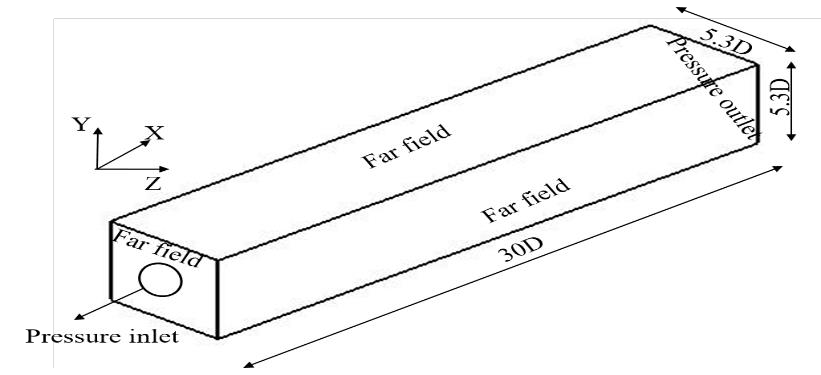
\includegraphics[width=3.4in]{domain.png}
\caption{Computational domain with boundary conditions}
\label{fig:domain}
\end{figure}
%%%%%%%%%%%%%%%%%%% FIGURE %%%%%%%%%%%%%%%%
\begin{figure}[h]
\centering
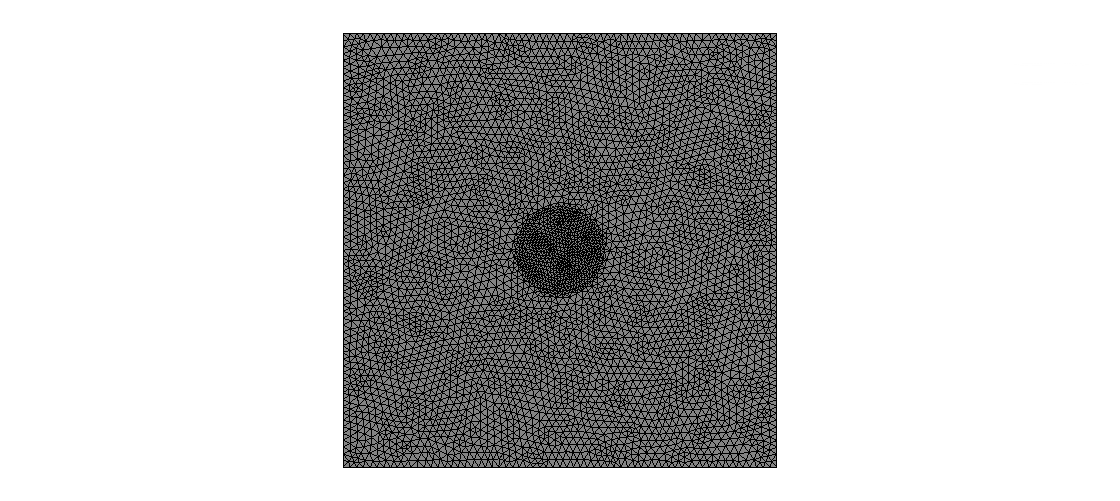
\includegraphics[width=3.4in]{mesh view.png}
\caption{Close-up view of coarse mesh near the exit of circular orifice}
\label{fig:mesh}
\end{figure}
%%%%%%%%%%%%%%%%%%% FIGURE %%%%%%%%%%%%%%%%

To validate the present numerical model, computed solutions of single and twin circular jets are compared with the numerical simulations and experimental measurements due to Anderson and Spall \cite{anderson2001experimental}. As shown in Table I, five different meshes with 0.8, 1.6, 2.7, 3.3, and 3.7 million cells are employed to check the grid dependency of the simulations. Fig. 5 clearly shows that mesh with 2.7 million or more elements produced almost identical results, and hence mesh size of 2.7 million is used for the present study. The results were obtained using quadrilateral cells generated in ANSYS Fluent Mesh.\textbf{ }Since the finer mesh size of 3.10 and 3.80 million showed no appreciable improvements in jet velocity predictions, a grid size of 2.7 million was used for all the cases of single and twin jet flow for the sake of computational ease. 

From Table II, the obtained circular single jet velocity with the \textit{SST K-$\omega$~}turbulence model matches the experimental and numerical work of Anderson and Spall \cite{anderson2001experimental}.~Fig. 6 shows the centreline velocity decay of a \textit{M} 0.8 jet for a single circular orifice jet. It is understood that the simulated numerical results of the \textit{SST K- $\omega$} turbulence model are similar to the experimental and numerical results of Anderson and Spall \cite{anderson2001experimental} and shown good agreement up to 10 jet diameters. Beyond 10\textit{D}, the predicted jet decay is slightly higher. Fig. 7 shows the velocity decay of a \textit{M} 0.8 jet along the symmetry plane for the twin circular orifice jets. The present numerical solution agrees reasonably well with the experimental results of Anderson and Spall \cite{anderson2001experimental} and Laban et al.\cite{laban2019experimental}.  The twin-jet profile also shows good agreement in all regions of the flow and matches well with the numerical data of Anderson and Spall \cite{anderson2001experimental}. 

%\begin{figure*}[ht]
%	\centering
%	\rule{\linewidth}{3cm}
%	\caption{Wide single column figure in a twocolumn document.}
%\end{figure*}

%\noindent \textbf{Table I}Grid independence test
\begin{table*}[ht]
	\caption{Grid independence test}
	\begin{centering}
	\begin{tabular}{|p{0.7in}|p{0.7in}|p{1.1in}|p{0.4in}|p{2.0in}|} \hline 
		\textbf{\textit{Mesh Name}} & \textbf{\textit{Element Size}} & \textbf{\textit{Mesh Size (Million)}} & \textbf{\textit{ U${}_{e}$}} & \textbf{\textit{Percentage Error = }}$\frac{{\boldsymbol{Ue}}_{\boldsymbol{New}\boldsymbol{\ }\boldsymbol{Mesh}\boldsymbol{-}\boldsymbol{\ }{\boldsymbol{Ue}}_{\boldsymbol{Old}\boldsymbol{\ }\boldsymbol{Mesh}}}}{{\boldsymbol{Ue}}_{\boldsymbol{New}\boldsymbol{\ }\boldsymbol{Mesh}}}\boldsymbol{\times }\boldsymbol{100}$\textbf{\textit{}} \\ \hline 
		M1 & 2.00 & 0.8 & 277.13 & - \\ \hline 
		M2 & 1.50 & 1.7 & 277.51 & 0.137 \\ \hline 
		M3 & 1.25 & 2.7 & 277.64 & 0.046 \\ \hline 
		M4 & 1.10 & 3.1 & 277.72 & 0.032 \\ \hline 
		M5 & 1.00 & 3.8 & 277.80 & 0.032 \\ \hline 
	\end{tabular}
	\par\end{centering}
\end{table*}


%%%%%%%%%%%%%%%%%%%%%%% insert two tables %%%%%%%%%%%%%%%%%%%%%%%%%%%%%%
\section{Results and Discussions}
The numerical study of single and twin jets with two different cross-sections is carried out, and the behaviour of twin jets is compared with that of a corresponding single jet. Whenever two jets enter into the atmosphere from the nozzle exit, the interaction between individual jets takes place rapidly. The mixing characteristics of any turbulent free jet flows are generally analysed by investigating the jet profile in streamwise (\textit{X}), lateral (\textit{Y}), and transverse (\textit{Z}) directions. For the present study, the two individual jets are adjacent to each other. Therefore, the velocity profiles of single and twin jet flows are studied in the \textit{X} direction alone. The flow properties of twin jets in the lateral and transverse directions are discussed in the future studies. The results have been plotted to bring out the effects of $S/D$ and orientation.  

Target tracking while maintaining a constant standoff distance from the target is called as standoff target tracking. It can be accomplished by a fixed-wing UAV by making it loitered around a target. The speed of the UAV should be more than the speed of the target as the fixed-wing UAV needs to maintain a forward motion to avoid stalling. In two dimensional (2D) plane it can be accomplished by a robot moving on the same plane or by a fixed-wing UAV loitering around the target in a circular path while keeping its altitude constant. There are different approaches available for target tracking in the existing literature. Kun et al. \cite{wu2017target} proposed modified non-singular fast terminal sliding mode for target tracking, and they proved the feasibility of trajectory with fast convergence through numerical results.   Ma et al. \cite{ma2010adaptive} proposed an inverse kinematic guidance with fast estimation scheme for the vision based tracking. Park \cite{park2016circling} proposed a simple, globally asymptotically stable relative side bearing angle based guidance law for circling over targets. Morgan \cite{quigley2005target} used super critical Hopf bifurcation concept to generate trajectories for the target tracking. 

The vector field based target tracking methods have been of increasing interest in recent days. In this method the desired course angles are generated as a function of position and the error in the course angle which forms the basis of the guidance law. Lawrence \cite{lawrence2003lyapunov} proposed Lyapunov vector field guidance (LVFG) for loitering in a circular path around a target.  In general, Lyapunov function is constructed to check the stability but, in the work first the Lyapunov function was chosen  considering the desired circle as a zero level set, and then stable vector fields were generated by ensuring that the time derivative of the Lyapunov function was negative.  Frew et al. \cite{frew2008coordinated} added phase keeping guidance to LVGF to propose a coordinated standoff target tracking. Hongda et al. \cite{chen2009tracking} proposed Tangent plus Lyapunov vector field guidance (T+LVFG) to achieve fast convergence to a standoff circle, and it was shown that the tangent vector field method outperformed the Lyapunov vector field \cite{lawrence2003lyapunov} if there existed a tangent to the circle. For better performance of target tracking, the desired trajectory should satisfy the curvature constraint of the vehicle. Pothen et al. \cite{pothen2017curvature} generated a curvature-constrained Lyapunov vector field where the generated path satisfied the maximum curvature limits and it showed faster convergence in comparison with Ref.~\citen{lawrence2003lyapunov}.  Oh et al. \cite{oh2014decentralised} added adaptive sliding mode concept to the existing T+LVFG technique to account the effect of remodeled disturbances in the autopilot loop. Shun et al. \cite{sun2019fast} proposed a fast convergence Lyapunov vector field guidance by using  off-line search algorithms.  

As discussed above a  wide variety of vector fields can be generated by the Lyapunov vector field framework for path following, target tracking and obstacle avoidance \cite{wilhelm2019vector, zhu2019evaluation} applications. However, constructing a simple vector field to guide vehicles for faster convergence to a desired standoff circle considering maneuverability constraints of a vehicle is still a challenging area as in many applications UAVs are initially deployed from sufficiently large distance away from the desired circle but the  the life of the battery of UAVs is limited. Hota et al. \cite{hota2009modified} and Alok et al. \cite{ranjanatime} solved the optimal path planning problem for converging to a straight line and a circle by using geometrical arguments but the curvature profile of the path is not continuous. This paper uses the findings of Ref.~\citen{ranjanatime} to generate a path with the novelty that it has a smooth curvature profile and is very close to the optimal path. The guidance law is also explicitly a function of the minimum turn radius of the vehicle, and hence it is applicable to different maneuverable vehicles. The other advantage of the algorithm is that the computation time is very fast, which makes it feasible for implementation in real-time as demonstrated through simulations.

\section{Problem Statement}

\begin{figure}[h]
	\centering
%	\includegraphics[width=3.4in]{scenario.PNG}
	\caption{Scenario of target tracking}
	\label{fig:geometry}
\end{figure}

In the fixed reference frame as shown in Fig. \ref{fig:geometry}, the target and the UAV are located at $\begin{pmatrix}
	x_{t} & y_{t}
\end{pmatrix}$ and $\begin{pmatrix}
x_{v} & y_{v}
\end{pmatrix}$, respectively. Here, $\boldsymbol{r_{v}}$ is the position vector of the UAV and $\boldsymbol{r_{t}}$  is the position vector of the target. The relative position vector of the UAV with respect to the target is denoted by $\boldsymbol{r}$  ($=\boldsymbol{r_{v}}-\boldsymbol{r_{t}}$). To converge to the circular path of radius $r_{d}$ as shown in the figure, a feasible Lyapunov guidance vector field ($\dot{\boldsymbol{r}}$) with an objective of faster convergence has to be constructed. This field can produce the reference course angle ($\chi_{d}$) commands to the higher-level control (guidance) loop. The guidance loop generates angular velocity commands, which should be followed by the vehicle for circular path convergence.

To study the performance of the circular path convergence the following kinematic equations of an unmanned vehicle are considered.
\begin{equation}\label{eq1}
\begin{split}
\dot{x}  = v_{a}\cos \psi +W_x\\
\dot{y}  = v_{a}\sin \psi+W_y
\end{split}
\end{equation} 
where, $v_a$ is the airspeed and  $\psi$ is the heading angle of the UAV.  $W_x$ and $W_y$ are the wind velocity components along the $X$ and $Y$ directions, respectively as shown in Fig. \ref{fig:geometryt}. It is assumed that altitude and airspeed are held constant by the control of longitudinal dynamics in line with the work presented in Ref.~\citen{nelson2007vector, liang2015combined} and \citen{frew2008coordinated}.


\begin{figure}[h]
\centering
%\includegraphics[width=3.4in]{rcc.png}
\caption{Velocity triangle}
\label{fig:geometryt}
\end{figure}

The kinematic equations \eqref{eq1} can be rewritten as \begin{equation}\label{eq1222}
\begin{split}
\dot{x}  = v_{g}\cos \chi \\
\dot{y}  = v_{g}\sin \chi
\end{split}
\end{equation}
where, $\chi$ is the course angle of the UAV. $v_g$  is the ground speed of the UAV, which is variable  even when the airspeed and the wind speed are constant. $v_g$ can be expressed as,
\begin{equation}\label{referec}
v_g=W_x\cos\chi+W_y\sin\chi+\sqrt{v_a^2+2W_xW_y\cos{\chi}\sin\chi}
\end{equation}
 To generate the guidance law, here we consider the first-order course angle dynamics as
\begin{align}
\mathop \chi \limits^.  &= \alpha ({\chi _d} - \chi ) &   ({\chi _d} - \chi) \in (\begin{matrix}
-\pi,~\pi
\end{matrix}] \label{eq:law}
\end{align}

where, $\alpha $ is the proportional gain. The relation between the course angle rate and the heading angle rate can be described as \cite{frew2008coordinated}

\begin{equation}\label{ratereln}
\dot{\chi} =F(\psi )\dot{\psi} 
\end{equation}
where, 

\begin{equation}\label{refereceee}
F(\psi)=\textstyle{\frac{v_a^{2}+v_a(W_x\cos\psi+W_y\sin\psi )}{v_a^{2}+W^{2}+2v_aW_x\cos\psi+2v_aW_y\sin\psi}}
\end{equation}

The heading rate constraints on the UAV can be imposed indirectly by constraining the course angle rate using \eqref{ratereln}. For  feasible operation $\sqrt{W_x^{2}+W_y^{2}}<v_a$ and hence, from \eqref{refereceee}, it can be observed that $F(\psi)\in(0.5,1]$. The course angle rate constraints can be set as $\dot{\chi}=0.5\dot{\psi}$ for safe operation. 


\section{Background}

In this section a brief review on the Lyapunov vector field based guidance for  unmanned vehicles is presented.

Lawrence et al.\cite{lawrence2007lyapunov} constructed the Lyapunov vector fields with the desired closed attractor as a globally asymptotically stable  limit cycle. It is done by considering the Lyapunov function, $V(\boldsymbol{r})$ such that on the desired attractor it has zero energy, elsewhere it has positive energy and also $V(\boldsymbol{r})$ is radially unbounded, that is, as $\boldsymbol{r}\rightarrow \infty , V(\boldsymbol{r})\rightarrow \infty$. 

The total time derivative of Lyapunov function is given by
\begin{equation}
\dot{V}(\boldsymbol{r})=\frac{\partial V}{\partial \boldsymbol{r}}\dot{\boldsymbol{r}}
\end{equation} 

For simpler analysis, without the loss of generality let us assume that the target is located at the origin so, $(\begin{matrix}
x_t,~y_t
\end{matrix})=(\begin{matrix}
0,~0
\end{matrix})$  and hence $\boldsymbol{r}$ is $\begin{bmatrix}
x_{v} &y_{v}
\end{bmatrix}$.

To ensure that the total time derivative of the Lyapunov function  is negative except on the attractor, the vector field ($\dot{\boldsymbol{r}}$) is defined as the sum of convergence $(A(\boldsymbol{r}))$ and circulation terms $(S(\boldsymbol{r}))$ as given below:
\begin{equation}
\dot{\boldsymbol{r}}=A(\boldsymbol{r})+S(\boldsymbol{r})
\end{equation} 

such that 
\begin{equation}\label{frac}
\frac{\partial V}{\partial \boldsymbol{r}}A(\boldsymbol{r})<0,
\end{equation}  

\begin{equation}\label{frac1}
\frac{\partial V}{\partial \boldsymbol{r}}S(\boldsymbol{r})=0
\end{equation}
and for a constant vector field
\begin{equation}\label{sqr}
\sqrt{A(\boldsymbol{r})^{2}+S(\boldsymbol{r})^{2}}=v_a
\end{equation}

$S(\boldsymbol{r})$ signifies the required modulation of the tangent curves of the vector field while converging to the desired attractor. 


Satisfying the equations, \eqref{frac} \eqref{frac1} and \eqref{sqr}, Lawrence et al. \cite{lawrence2003lyapunov} proposed a Lyapunov guidance vector field for a standoff target tracking, which can be described as
\begin{equation}
\left[ {\begin{array}{*{20}{c}}
	{\dot{x}_{d} } \\ 
	{\dot{y}_{d} } 
	\end{array}} \right] = \left[ {\begin{array}{*{20}{c}}
	{ - \frac{{{r^2} - {r_d}^2}}{{{r^2} + {r_d}^2}}x_v - \frac{{2r{r_d}}}{{{r^2} + {r_d}^2}}y_v} \\ 
	{ - \frac{{{r^2} - {r_d}^2}}{{{r^2} + {r_d}^2}}y_v + \frac{{2r{r_d}}}{{{r^2} + {r_d}^2}}x_v} 
	\end{array}} \right]
\end{equation} where,  $r~ (= {{\boldsymbol{r}}^T}{\boldsymbol{\hat r}}) $ is the horizontal range between the unmanned vehicle and the target on the loitering plane. $\dot{x}_{d}$ and $\dot{y}_{d}$ are the desired inertial velocity components along  $X$-axis and $Y$-axis, respectively. The unit vector in the direction of $\boldsymbol{r}$ is represented by $\hat{\boldsymbol{r}}$.


Similarly, by modifying the circulation term for faster convergence Pothen et al.\cite{pothen2017curvature} proposed a curvature constrained Lyapunov guidance vector field, which can be described as  
\begin{equation}
\begin{footnotesize}
\left[ {\begin{array}{*{20}{c}}
	{\dot{x}_{d} } \\ 
	{\dot{y}_{d} } 
	\end{array}} \right] = \frac{{ - v_a}}{{\sqrt {{r^4} + ({c^2} - 2){r_d}^2{r^2} + {r_d}^4} }}\left[ {\begin{array}{*{20}{c}}
	{\frac{{{r^2} - {r_d}^2}}{r}x_v + c{r_d}y_v} \\ 
	{\frac{{{r^2} - {r_d}^2}}{r}y_v - c{r_d}x_v} 
	\end{array}} \right]
	\end{footnotesize}
\end{equation} where, 
\[c = \left\{ {\begin{array}{*{20}{c}}
	{\frac{r}{{{r_d}}}}  \quad \textrm{if} \quad r<{r_d}\\ 
	{\frac{{{r_d}}}{r}}  \quad \textrm{if} \quad r \ge {r_d}
	\end{array}} \right.\]


\section{ Proposed Lyapunov Vector Field}

In this section, a new guidance vector field is proposed using the Lyapunov vector field guidance approach  for faster convergence to the standoff circle. The objective is to generate the path which is of smooth curvature profile satisfying the maximum curvature limit of a fixed-wing vehicle  and the length of the path should be close to the optimal one. For this, a positive definite scalar valued function $V({\bf{r}})$ is considered by treating the desired standoff circle with respect to the target as a zero level set, which is given below:
\begin{equation}
V(\boldsymbol{r}) = {(r - {r_d})^2}
\end{equation}

The total time derivative of the Lyapunov function is given by
\begin{equation}
\dot{V}(\boldsymbol{r})=\frac{\partial V}{\partial \boldsymbol{r}}\frac{d\boldsymbol{r}}{dt}
\end{equation} where,
\begin{equation} \label{partial}
\begin{split}
\frac{\partial V}{\partial \boldsymbol{r}} &= \begin{bmatrix}
\frac{\partial V}{\partial x_{v}} &\frac{\partial V}{\partial y_{v}} 
\end{bmatrix} \\
& = \dfrac{2(r-r_{d})}{r}\begin{bmatrix}
x_{v} &y_{v}
\end{bmatrix}\\
& = \dfrac{2(r-r_{d})}{r}\boldsymbol{r}\\
& = 2(r-r_{d})\hat{\boldsymbol{r}}
\end{split}
\end{equation}
The desired vector field, $\dot{\boldsymbol{r}}$, can be defined as the sum of the convergence $({f_1})$ and circulation $({f_2})$ components given below and they should be selected in such a manner that the total time derivative of the Lyapunov function, $\dot{V}(\boldsymbol{r})$, is negative definite.
\begin{equation}\label{rdot1}
\dot{\boldsymbol{r}} =- {f_1}\hat{\boldsymbol{r}}^{T}\pm {f_2}\hat{\boldsymbol{n}} \times \hat{\boldsymbol{r}}^{T}
\end{equation} where, $\hat{\boldsymbol{n}}$ is the unit normal vector to the loitering plane.  There are two possible normal vectors: i) the positive convention is to indicate the normal vector which points up-side of the loitering plane, ii) the negative convention is to indicate the normal vector which points downside of the loitering plane.

Here, the convergence $({f_1})$ and circulation $({f_2})$ terms are normalized odd and even functions of $({r-{r_d}})$. They are defined by decomposing an exponential  function, ${a^{c(r - {r_d})}}$, into odd and even functions, and are normalized with the desired speed of the vehicle to generate a constant speed vector field as expressed below,
\begin{equation}\label{f1}
{f_1} =v_{g}\frac{{{a^{c(r - {r_{d}})}} - {a^{ - c(r - {r_{d}})}}}}{{{a^{c(r - {r_{d}})}} + {a^{ - c(r - {r_{d}})}}}}
\end{equation}
\begin{equation}\label{f2}
{f_2} =v_{g}\frac{2}{{{a^{c(r - {r_d})}} + {a^{ - c(r - {r_d})}}}}
\end{equation} where, the base of the exponential function, $a$, can be any positive constant greater than 1 and $c$ is the control parameter which will be designed later to satisfy the curvature bounds. Using \eqref{f1} and \eqref{f2}, the equation \eqref{rdot1} can be written as, 
\begin{multline}\label{rdott0}
\dot{\boldsymbol{r}} =  - v_{g}\frac{{{a^{c(r - {r_d})}} - {a^{ - c(r - {r_d})}}}}{{{a^{c(r - {r_d})}} + {a^{ - c(r - {r_d})}}}}\hat{\boldsymbol{r}}^{T}\\ \pm v_{g}\frac{2}{{{a^{c(r - {r_d})}} + {a^{ - c(r - {r_d})}}}}\hat{\boldsymbol{n}} \times \hat{\boldsymbol{r}}^{T}
\end{multline}

Here,
\begin{equation}
\hat{\boldsymbol{n}} \times \hat{\boldsymbol{r}}^{T}=\begin{bmatrix}
\cos(\frac{\pi}{2}) & -\sin(\frac{\pi}{2})\\ 
\sin(\frac{\pi}{2}) & \cos(\frac{\pi}{2})
\end{bmatrix}\left[ {\begin{array}{*{20}{c}}
	\boldsymbol{\hat x}_v\\
	\boldsymbol{\hat y}_v
	\end{array}} \right] 
\end{equation}
So, $\dot{\boldsymbol{r}}$ in \eqref{rdott0} will become
\begin{multline}\label{rdott}
\dot{\boldsymbol{r}} =  - v_{g}\frac{{{a^{c(r - {r_d})}} - {a^{ - c(r - {r_d})}}}}{{{a^{c(r - {r_d})}} + {a^{ - c(r - {r_d})}}}}\left[ {\begin{array}{*{20}{c}}
	\boldsymbol{\hat x}_{v}\\
	\boldsymbol{\hat y}_{v}
	\end{array}} \right] \\ \pm v_{g}\frac{2}{{{a^{c(r - {r_d})}} + {a^{ - c(r - {r_d})}}}}\left[ {\begin{array}{*{20}{c}}
	\boldsymbol{-\hat y}_{v}\\
	\boldsymbol{\hat x}_{v}
	\end{array}} \right]
\end{multline}

For clockwise loitering, the desired vector field can be represented in the Cartesian coordinate as
\begin{equation}\label{referece}
\begin{split}
\textstyle\dot{x}_{d}  =  - \frac{v_{g}}{r}\frac{{{a^{c(r - {r_d})}} - {a^{ - c(r - {r_d})}}}}{{{a^{c(r - {r_d})}} + {a^{ - c(r - {r_d})}}}}x_v +\frac{v_{g}}{r}\frac{2}{{{a^{c(r - {r_d})}} + {a^{ - c(r - {r_d})}}}}y_v \\
\textstyle\dot{y}_{d}  =  - \frac{v_{g}}{r}\frac{{{a^{c(r - {r_d})}} - {a^{ - c(r - {r_d})}}}}{{{a^{c(r - {r_d})}} + {a^{ - c(r - {r_d})}}}}y_v - \frac{v_{g}}{r}\frac{2}{{{a^{c(r - {r_d})}} + {a^{ - c(r - {r_d})}}}}x_v
\end{split}
\end{equation}

The vector field in \eqref{referece} forms the desired circle as an asymptotically stable limit cycle. The vectors of this field give the desired course angles as a function of position to follow the desired limit cycle. The expression for the desired course angle is,
\begin{equation}
{\chi _ {d}} = \arctan \left( {\frac{{\dot{y}_{d} }}{{\dot{x}_{d} }}} \right)
\end{equation}
Using \eqref{referece} the above equation becomes,
\begin{equation}
{\chi _{d}} = \arctan \left( {\frac{{\left( {{a^{c(r - {r_d})}} - {a^{ - c(r - {r_d})}}} \right)y_v - 2x_v}}{{\left( {{a^{c(r - {r_d})}} - {a^{ - c(r - {r_d})}}} \right)x_v + 2y_v}}} \right)
\end{equation}

The curvature ($\kappa = \frac{{{{\dot \chi }_d}}}{v_{g}}$) of the path developed by these vector fields is, 

\begin{equation}\label{eq15}
\kappa = \frac{2}{{{a^{c(r - {r_d})}} + {a^{ - c(r - {r_d})}}}}\left[ {c\ln (a)\frac{{{a^{c(r - {r_d})}} - {a^{ - c(r - {r_d})}}}}{{{a^{c(r - {r_d})}} + {a^{ - c(r - {r_d})}}}} - \frac{1}{r}} \right]
\end{equation}

\subsection{Stationary Target Tracking}
Alok et al.\cite{ranjanatime} generated optimal paths for convergence to the desired circle from different initial positions and orientations. It was shown there that if the initial position was sufficiently far from the circular path to be followed, the straight-line segment of the optimal CSC (Circular path of minimum turn radius- Straight line- Circular path  of minimum turn radius) path should pass through the center of the circle, which is shown in Fig.   \ref{fig:dubin}. In this figure the UAV with a minimum turn radius of $r_{\min }$  converges to the circular path of radius ${r_d}$  starting from the location $(x_0,y_0)$.
Here, $d$ and $\theta$ are defined as,
\begin{equation}
d = ({r_{\min }} + {r_d})\cos {\theta} 
\end{equation}
\begin{equation}
\theta  = \arcsin\left( {\frac{{{r_{\min }}}}{{{r_{\min }} + {r_d}}}} \right)
\end{equation}
For optimal time convergence to the desired circular path the following properties can be observed:

\noindent
Region 1. if $r > d$, the guidance law for optimal convergence is composed of the convergence term only.
\\Region 2. if $r_d< r\leq d$, the guidance law for optimal convergence is composed of both the convergence and the circulation terms.
\\Region 3. if $r={r_d}$, the guidance law for optimal convergence is composed of the circulation term only.

The profiles of convergence and circulation terms in case of optimal time convergence are analyzed here  by rewriting \eqref{rdott} as given below:
\begin{equation}
\begin{bmatrix}
\dot{x}_v\\ \dot{y}_v

\end{bmatrix}=\begin{bmatrix}
-\hat{x}_v &\hat{y}_v \\ 
-\hat{y}_v& -\hat{x}_v
\end{bmatrix}\begin{bmatrix}
f_{1}\\f_{2} 

\end{bmatrix}
\end{equation}

This gives,
\begin{equation}\label{eq16}
\begin{bmatrix}
f_{1}\\ f_{2}
\end{bmatrix}=\begin{bmatrix}
-\frac{x_v}{r} & -\frac{y_v}{r}\\ 
\frac{y_v}{r} & -\frac{x_v}{r}
\end{bmatrix}\begin{bmatrix}
\dot{x}_v \\  \dot{y}_v
\end{bmatrix}
\end{equation}

\begin{figure}[t!]
	\centering
%	\includegraphics[width=3.4in]{alok2.PNG}
	\caption{ Dubins path with zero initial orientation angle}
	\label{fig:dubin}
\end{figure}


\begin{figure}[t!]
	\centering
%	\includegraphics[width=3.4in]{alok_plot.eps}
	\caption{Variation of the convergence and circulation terms for optimal convergence}
	\label{fig:conn}
\end{figure}

To visualize the variations of convergence and circulation terms with respect to $r$, an example is considered here with the following data: $x$=$-1.5$ $m$ , $y$=$0$ $m$, $r_{d}=0.5$ $m$, $r_{min}=0.3$ $m$ and  $v_a=0.2$ $m/s$.  The profiles of these two terms for optimal convergence are plotted in Fig. \ref{fig:conn}.

But the main problem to adopt the optimal CSC path for implementation is that the curvature profile of the path is not continuous, which makes it difficult for tracking by fixed-wing UAVs. This motivates us to choose the control parameter, $c$, of our guidance algorithm in such a way that it generates a smooth path and the length of which is very close to the optimal one.


 \subsection{ Proposed Control Parameter, c}

The convergence term, ${f_1}$  of \eqref{f1} and the circulation term, ${f_2}$  of \eqref{f2} can also be written as
\begin{equation}
{f_1} = v_{a}\tanh (c(r - {r_d})\ln (a))
\end{equation}

\begin{equation}
{f_2} = v_{a}{\mathop{\rm sech}\nolimits} (c(r - {r_d})\ln (a))
\end{equation}
Let us define, $m=c(r - {r_d})\ln (a)$.
The variations of the convergence and the circulation functions with the variable $m$ of the proposed guidance law is depicted in Fig. \ref{fig:hyperbolic }.

As stated above for optimal convergence, switching from Region 1 to Region 2, should occur at $r=d$. So the value of $m$ at the transition, defined as $k$, will be expressed as

\begin{equation}
{c}({{d - {r_d}}})\ln{a}=k
\end{equation}
which gives the control parameter, $c$ as,
\begin{equation}\label{cdesign}
c = \frac{k}{({{d - {r_d}}})\ln{a}}
\end{equation}

A trade-off between the feasibility and the optimality is made to choose the constant, $k$ which can be of any value in the range ($0$,~$4$) as shown in  Fig. \ref{fig:hyperbolic }. The exact value of this can be selected using an optimization algorithm for the nonlinear multivariable function \eqref{eq15}.

Let us define, $k_1=({{d - {r_d}}})\ln{a}$. Note that for given $r_d$ and $r_{min}$, $k_1$ is a constant. The equation, \eqref{eq15} can be re-written as 


\begin{equation}
\begin{split}
\kappa(r,k)= & \frac{2}{{{a^{\frac{k}{k_1}(r - {r_d})}} + {a^{ - \frac{k}{k_1}(r - {r_d})}}}}~~~~~~~\\
~~~~~~~& ~~\left[ {\frac{k}{k_1}\ln (a)\frac{{{a^{\frac{k}{k_1}(r - {r_d})}} - {a^{ - \frac{k}{k_1}(r - {r_d})}}}}{{{a^{\frac{k}{k_1}(r - {r_d})}} + {a^{ - \frac{k}{k_1}(r - {r_d})}}}} - \frac{1}{r}} \right]
\end{split}
\end{equation}




The optimization problem can be formulated as

\begin{equation}
\max~\kappa (r,k)
~~~\mathrm{such~that}~~  \left\{ {\begin{array}{*{20}{c}}
	{\kappa(r,k)}-\kappa_{max}=0\\ 
	r_{lb} \leq r\leq r_{up}
\\ 
	k_{lb} \leq k\leq k_{up}
	\end{array}} \right.
\end{equation}
where, $r_{lb}$ and $k_{lb}$ are the lower bounds of $r$ and $k$, respectively. And $r_{ub}$ and $k_{ub}$ are the upper bounds of  $r$ and $k$, respectively. $\kappa_{max}=\frac{1}{r_{min}}$, is the maximum curvature bound of the UAV. The nonlinear programming solver `fmincon' in MATLAB is used to solve the optimization problem to find out the optimal value of $k$. The above analysis holds good for convergence when the initial position is outside the standoff circle.

\begin{figure}[t!]
	\centering
%	\includegraphics[width=3.4in]{in_draw}
	\caption{ Optimal path of converging from inside standoff circle}
	\label{fig:dubii}
\end{figure}

Similar analysis can be done if the initial position is inside the standoff circle as shown in  Fig. \ref{fig:dubii}. In that case, the parameter, $c$, should be selected as
\begin{equation}
c = \frac{l}{d_1- {r_d}}
\end{equation}
here, $l$ is a positive constant similar to $k$ and in the range of ($0$,~ $4$). $d_1$ can be defined as 
\begin{equation}
d_1=({r_d}-r_{min})\cos \beta 
\end{equation} where,
\begin{equation}
\beta  = \arcsin\left( {\frac{{{r_{\min }}}}{{{r_{d }} - {r_{\min }}}}} \right)
\end{equation}


\begin{figure}[t!]
	\centering
%	\includegraphics[width=3.4in]{tanh.eps}
	\caption{Circulation and convergence functions in the proposed guidance law}
	\label{fig:hyperbolic }
\end{figure}



\subsection{Stability Analysis}

The stability of the attractor set $(r-r_{d}=0)$ of the system (\ref{referece}) can be  analysed with the help of Lyapunov direct method. The Lyapunov  function,  $V(\boldsymbol{r})$ is choosen to satisfy the following conditions:

\begin{itemize}
	\item $V(\boldsymbol{r})=0$, for $r=r_{d}$
	\item $V(\boldsymbol{r})> 0$, for all $r\neq r_{d}$
	\item $V(\boldsymbol{r})$ is radially unbounded, which implies  $V(\boldsymbol{r})\rightarrow \infty$ if $r\rightarrow \infty$.
\end{itemize}	
		
The total time derivative of the Lyapunov function is
\begin{equation}
\dot{V}(\boldsymbol{r})=\frac{\partial V}{\partial \boldsymbol{r}}\frac{d\boldsymbol{r}}{dt}
\end{equation}

Using (\ref{partial}) and (\ref{rdot1}) 
\begin{equation}
\dot{V}(\boldsymbol{r}) =2(r-r_{d})\begin{bmatrix}
	\hat{x} & \hat{y}
\end{bmatrix}\left[{-f_{1}\begin{bmatrix}
		\hat{x}\\ \hat{y}
		
\end{bmatrix}} \pm {f_{2}\begin{bmatrix}
		-\hat{y}\\ \hat{x}
		
\end{bmatrix}}\right]
\end{equation}

\begin{equation}
\dot{V}(\boldsymbol{r})=-2(r-r_{d})f_{1}
\end{equation}

As the function, $f_{1}$, is an odd function of $(r-r_d)$

\begin{equation}
\dot{V}(\boldsymbol{r}) < 0 , \quad \textrm{for all} \quad r\neq r_{d}  
\end{equation}
Hence, in the sense of Lyapunov, the attractor set $(r-r_{d}=0)$ is globally asymptotically stable. 



\subsection{Feasibility Analysis}

Using \eqref{eq15}, the curvature of the tangent curves of the proposed vector field is analyzed. In general, for feasible tracking operation, the path should be designed in such a way that it takes into account the dynamic constraints of the vehicle. Some of these constraints can be imposed by applying constraints on the curvature of the developed path. From \eqref{eq15} and \eqref{cdesign}, it can be seen that for a constant speed vehicle, the curvature of the proposed vector field is only the function of one scaling parameter, that is, $k$.

For converging from the outside of the circular path, the minimum turn radius of the vehicle should be less than or equal to the radius of the standoff circle to which the vehicle will converge. When the minimum turn radius of the vehicle is equal to the radius of the standoff circle, the value of the scaling parameter ($k$) is 2.2 which is the the upper bound. The lower bound of $k$ is computed using `fmincon' function in MATLAB to find the value as 2. 

For converging from the inside of the circular path, the minimum turn radius of the vehicle should be one-third of the standoff circular path to be followed as in Ref.~\citen{pothen2017curvature}. In this case, the upper and lower bounds on the scaling parameter, $l$, are $2$ and $1.5$, respectively, which is computed in the similar way of finding out $k$. It is found that the proposed algorithm outperforms \cite{pothen2017curvature} and \cite{lawrence2003lyapunov} even with the lower bounds of $k$ and $l$.  

\subsection{Moving Target Tracking}

The above said concept is now extended for tracking a moving target.  To study the performance let us consider the dynamics of the target be as follows:
\begin{equation}\label{eq78}
\begin{split}
\dot{x_t}  = v_{tx}\\
\dot{y_t}  = v_{ty}
\end{split}
\end{equation}
 where, $v_{tx}$ and $v_{ty}$ are the velocity components of the target in the directions of $X$ and $Y$ axes, respectively, and let us assume that these are known. Moving target tracking is achieved by tracking the moving target position, $(x_t,~  y_t)$ at every moment. We have seen that for the stationary target tracking equation number \eqref{referece} is the Lyapunov guidance vector field where the target was considered at the origin, $(0,~0)$ for simplicity but without the loss in generality. The same vector field is used here for the moving target tracking problem by shifting the origin to the target position at each instance. To achieve it,  $x_v$ and $y_v$ are replaced with $x_v-x_t$ and $y_v-y_t$, respectively, so \eqref{referece} will become,
 \begin{multline}\label{referece1}
\begin{aligned}
\dot{x}_{d}  =  - \frac{v_{a}}{r}\frac{{{a^{c(r - {r_d})}} - {a^{ - c(r - {r_d})}}}}{{{a^{c(r - {r_d})}}+ {a^{ - c(r - {r_d})}}}}(x_v-x_t) \\+\frac{v_{a}}{r}\frac{2}{{{a^{c(r - {r_d})}} + {a^{ - c(r - {r_d})}}}}(y_v-y_t) \\  \dot{y}_{d}  =  - \frac{v_{a}}{r}\frac{{{a^{c(r - {r_d})}} - {a^{ - c(r - {r_d})}}}}{{{a^{c(r - {r_d})}} + {a^{ - c(r - {r_d})}}}}(y_v-y_t) \\- \frac{v_{a}}{r}\frac{2}{{{a^{c(r - {r_d})}} + {a^{ - c(r - {r_d})}}}}(x_v-x_t)
\end{aligned}
\end{multline}

where, $r=\sqrt{(x_v-x_t)^2+(y_v-y_t)^2}$.

\section{Simulation Results}

\subsection{Stationary Target Tracking}

In this section, simulation results are presented to validate the proposed Lyapunov vector field guidance law, using the kinematic model of the vehicle (\ref{eq1}) with the following simulation data: 

The maximum curvature limit of the vehicle is $\kappa =\frac{1}{r_{min}}=0.0143$  $m^{-1}$. The  airspeed is ${v_a}= 15$ $m/s$ \cite{Aviones:UAVFlightSimulator}-\cite{hota2014optimal}, and a wind  of velocity $W=(5~~5)~m/s$ is considered for each case. The vehicle has a guidance loop \eqref{eq:law} with control gain ${\alpha} = 10$. The target is located at $\begin{pmatrix}
0 & 0
\end{pmatrix}~m$ and  the initial position of the UAV is  $\begin{pmatrix}
-300 & 0
\end{pmatrix}~m$. The desired standoff distance is considered as ${r_d}=100$ $m$.

The same data are also considered for generating paths using guidance laws in the existing literature (Ref.~\citen{lawrence2003lyapunov} and \citen{pothen2017curvature}) to compare and to establish the superiority of the proposed guidance algorithm.


\begin{figure}[htpb]
	\begin{subfigure}{0.5\textwidth}
	\centering
%	\includegraphics[width=3.3in]{D_one.eps}
	\caption{Trajectories for stationary target tracking}
	\label{fig:traj}
\end{subfigure}
\begin{subfigure}{0.5\textwidth}
	\centering
%	\includegraphics[width=3.3in]{D_two.eps}
	\caption{Curvature variation}
	\label{fig:comp}
\end{subfigure}
\begin{subfigure}{0.5\textwidth}
	\centering
%	\includegraphics[width=3.3in]{D_three.eps}
	\caption{Convergence time}
	\label{fig:time}
\end{subfigure}
\caption{Stationary target tracking when the UAV starts from outside of the standoff circle}
\label{fig:fig_five}
\end{figure}




Fig. \ref{fig:traj} shows UAV trajectories generated by the proposed guidance field along with the algorithms presented in Ref.~\citen{lawrence2003lyapunov} and \citen{pothen2017curvature}. It shows all the three trajectories converge and follow the standoff circle whose center is the location  of the stationary target.  The curvature variation of guidance vector fields while converging from outside of the standoff circle is shown in Fig. \ref{fig:comp}, which shows that the curvature limit is also satisfied. Fig. \ref{fig:time} shows the time required to converge to the circular path. It is clearly seen that the time taken by the proposed guidance law  is  lower in comparison to the work presented in Ref.~\citen{lawrence2003lyapunov} and Ref.~\citen{pothen2017curvature}. With the proposed guidance law, the convergence time  of the UAV is $17$ $sec$, whereas , it is $23$ $sec$ with the guidance algorithm in Ref.~\citen{pothen2017curvature} and $40$ $sec$ with the guidance algorithm in Ref.~\citen{lawrence2003lyapunov}.


It is to mention that the proposed guidance vector field (\ref{referece}) has a singular point at the center of the standoff circle as at $r=0$, the curvature is not defined but it has no practical implication.



\begin{figure}[htpb]
	\begin{subfigure}{0.5\textwidth}
	\centering
%	\includegraphics[width=3.3in]{D_four.eps}
	\caption{Stationary target tracking from inside standoff circle}
	\label{fig:inside}
	
\end{subfigure}
\begin{subfigure}{0.5\textwidth}
	\centering
%	\includegraphics[width=3.3in]{D_five.eps}
	\caption{Curvature variation}
	\label{fig:k2}
	
\end{subfigure}
\begin{subfigure}{0.5\textwidth}
	\centering
%	\includegraphics[width=3.3in]{D_six.eps}
	\caption{Converging time profile}
	\label{fig:time2}
\end{subfigure}
\caption{Stationary target tracking}
\label{fig:fig_four}
\end{figure}



As the algorithm \cite{pothen2017curvature} is constrained by $r_d\geqslant\dfrac{3.0126}{\kappa_{max}}$, for case studies when the UAV starts from the inside of the standoff circle, the radius of the circular path is considered as  ${r_d}=220$ $m$ . The initial position is considered as $\begin{pmatrix}
5 & 0
\end{pmatrix}~m$.
Fig. \ref{fig:inside},  Fig. \ref{fig:k2} and Fig. \ref{fig:time2} show trajectories, the curvature variation and the time required to converge to the circular path for all three algorithms, respectively. It is seen that the performance of the proposed algorithm is far better.



\begin{figure}[htpb]
	\centering
%	\includegraphics[width=3.5in, height=1.7in]{D_seven.eps}
	\caption{Trajectories for different initial orientation angles}
	\label{fig:diff}
\end{figure}
In real-time scenarios, the control input gets saturated when it crosses its maximum bound. Such a situation is also considered here by setting the initial orientation angles as shown in Fig. \ref{fig:diff}. The initial circular arcs indicate the saturation of the control signal. 


\begin{figure}[htpb]
	\begin{subfigure}{0.5\textwidth}
	\centering
%	\includegraphics[width=3.5in, height=2in]{D_eight.eps}
	\caption{Trajectories for three different vehicles}
	\label{fig:rmin}
	
	\end{subfigure}
\begin{subfigure}{0.5\textwidth}
	\centering
%	\includegraphics[width=3.5in, height=2in]{D_nine.eps}
	\caption{Curvature analysis of three different vehicles}
	\label{fig:kappa for different}
\end{subfigure}
\caption{Stationary target tracking}
\label{fig:fig_three}
\end{figure}


Fig. \ref{fig:rmin} shows trajectories for four different vehicles with different values of minimum radius of curvature ($50~m$, $60~m$, $70~m$ and $80~m$, respectively). The corresponding scaling parameters ($k$) are obtained by using `fmincon' of MATLAB  and the values are, $2.1346$, $2.15$, $2.1634$, and $2.1751$, respectively. Corresponding curvature plots are shown in Fig. \ref{fig:kappa for different}. From the figure it can be clearly seen that all the trajectories are within their respective curvature bounds. This implies that the proposed guidance algorithm is equally applicable for different vehicles with different maneuvering capabilities.

If the wind is time varying, the algorithm will still be useful to generate the paths for standoff target tracking. Let us consider an example of variable wind case where the wind model is similar to the model used in Ref.~\citen{hota2014time}, which is given below:
\begin{equation}\label{raterelnpp-}
W=a+b\sin \frac{\pi t}{T}
\end{equation}
where, the constants are $a=5$, $b=1$, $T=10$, from which $W_x$ and $W_y$ can be expressed as
\begin{equation}\label{raterelnpp}
W_x(t)=W_y(t)=\frac{a}{\sqrt{2}}+\frac{b}{\sqrt{2}}\sin \frac{\pi t}{T}
\end{equation}  

With the above said wind condition, the path has been generated as shown in Fig. \ref{fig:diffgg} for different initial poses.  In all the cases it can be seen that the paths converge to the desired circular path.

\begin{figure}[htpb]
	\centering
%	\includegraphics[width=3.5in, height=3.8in]{g_and_g.eps}
	\caption{Stationary target tracking in variable wind condition for different initial poses} 
	\label{fig:diffgg}
\end{figure}

\subsection{Moving Target Tracking}
Let us consider the case when the target is moving with a velocity of $\begin{pmatrix}
7.5 & 7.5 \end{pmatrix}~m/s$ from the origin as shown in Fig. \ref{fig:targ}. Let us assume that the UAV with the airspeed of $15~m/s$ from the starting position  $\begin{pmatrix} - 350& 0 \end{pmatrix}~m$ has to track the moving target while maintaining the standoff distance of $220~m$. Fig. \ref{fig:targ} shows trajectories of the UAV while tracking the target. Corresponding range plot between the UAV and the target is shown in Fig. \ref{fig:targ_time}, which shows that the deviation from the standoff distance is about $30$ $m$ at steady state, which is due to the constant linear speed input and nonholonomic constraints of the UAV. The curvature plot of the  trajectory of the UAV is depicted in Fig. \ref{fig:ka} to illustrate that the curvature of the designed trajectory is within its maximum curvature bounds.

\begin{figure}[htpb]
	\begin{subfigure}{0.5\textwidth}
	\centering
%	\includegraphics[width=3.2in]{dd_ten.eps}
	\caption{Moving target tracking}s
	\label{fig:targ}
	\end{subfigure}
\begin{subfigure}{0.5\textwidth}
	\centering
%	\includegraphics[width=3.2in]{dd_ele.eps}
	\caption{Moving target tracking time profile}
	\label{fig:targ_time}
	\end{subfigure}
\begin{subfigure}{0.5\textwidth}
	\centering
%	\includegraphics[width=3.3in]{dd_twe.eps}
	\caption{Curvature analysis }
	\label{fig:ka}
\end{subfigure}
\caption{Moving target tracking}
\label{fig:fig_two}
\end{figure}



\section{Conclusion}

A fast convergence guidance algorithm based on the Lyapunov guidance vector field theory for standoff target tracking by  UAVs has been presented in this work for both stationary and moving targets in the presence of wind.  The proposed guidance law is explicitly a function of the minimum turn radius of the vehicle, and hence it is applicable to different maneuverable vehicles.  The proposed law has been compared with other LVGF based algorithms in literature  to show its faster convergence performance.  The other advantage of the algorithm is that it generates a smooth near optimal path in lower time in comparison to the similar work in the literature, which makes it feasible for real-time applications. The work can be extended to perform real-time target tracking by  UAVs in  3-dimensional environments. 

\bibliographystyle{SageV}
\bibliography{Bibliography}

\end{document}
